% Source: physical PDF p. 310 (printed p. 287). Coverage: Figure 20.3 and complete caption. Uncertainty: none; outer fermion loop, two external gauge-boson lines, diagonal gauge-boson line, and five fermion bubbles reconstructed from the rendered source.
\begin{figure}[htbp]
 \centering
 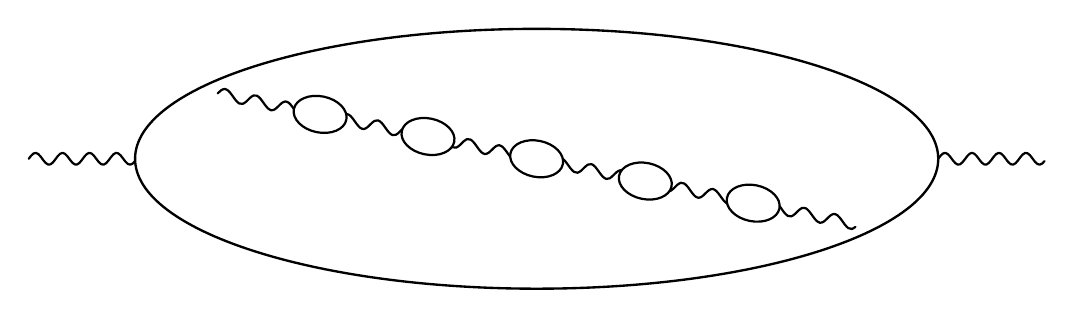
\begin{tikzpicture}[x=1cm,y=1cm,line cap=round,line join=round]
  % The large closed fermion loop.
  \draw[line width=0.85pt] (0,0) ellipse[x radius=5.1,y radius=1.65];

  % External gauge-boson lines entering and leaving at the loop's midpoints.
  \draw[line width=0.8pt,smooth,samples=45,domain=-6.45:-5.1]
   plot (\x,{0.075*sin(1050*(\x+6.45))});
  \draw[line width=0.8pt,smooth,samples=45,domain=5.1:6.45]
   plot (\x,{0.075*sin(1050*(\x-5.1))});

  % The diagonal gauge-boson line that carries the chain of vacuum-polarization bubbles.
  \draw[line width=0.8pt,smooth,samples=180,domain=-4.05:4.05]
   plot (\x,{-0.205*\x+0.075*sin(930*(\x+4.05))});

  % Five closed fermion bubbles inserted along the diagonal gauge-boson line.
  \foreach \x in {-2.75,-1.38,0,1.38,2.75}{
   \begin{scope}[shift={({\x},{-0.205*\x})},rotate=-11.6]
    \fill[white] (0,0) ellipse[x radius=0.34,y radius=0.23];
    \draw[line width=0.8pt] (0,0) ellipse[x radius=0.34,y radius=0.23];
   \end{scope}
  }
 \end{tikzpicture}
 \renewcommand{\thefigure}{20.3}
 \caption{One of a class of $N$-loop Feynman diagrams that grow as $N!$. Solid lines are fermions; wavy lines are gauge bosons.}
 \label{fig:20.3}
\end{figure}
